\newpage
\section{Resultados}

Os resultados foram obtidos para cada filtro.

\subsection{FPB}

A resposta em frequência para o filtro passa-baixas é mostrada na figura \ref{fRFPB}.

\begin{figure}[H]
 \centering
 \label{fRFPB}
 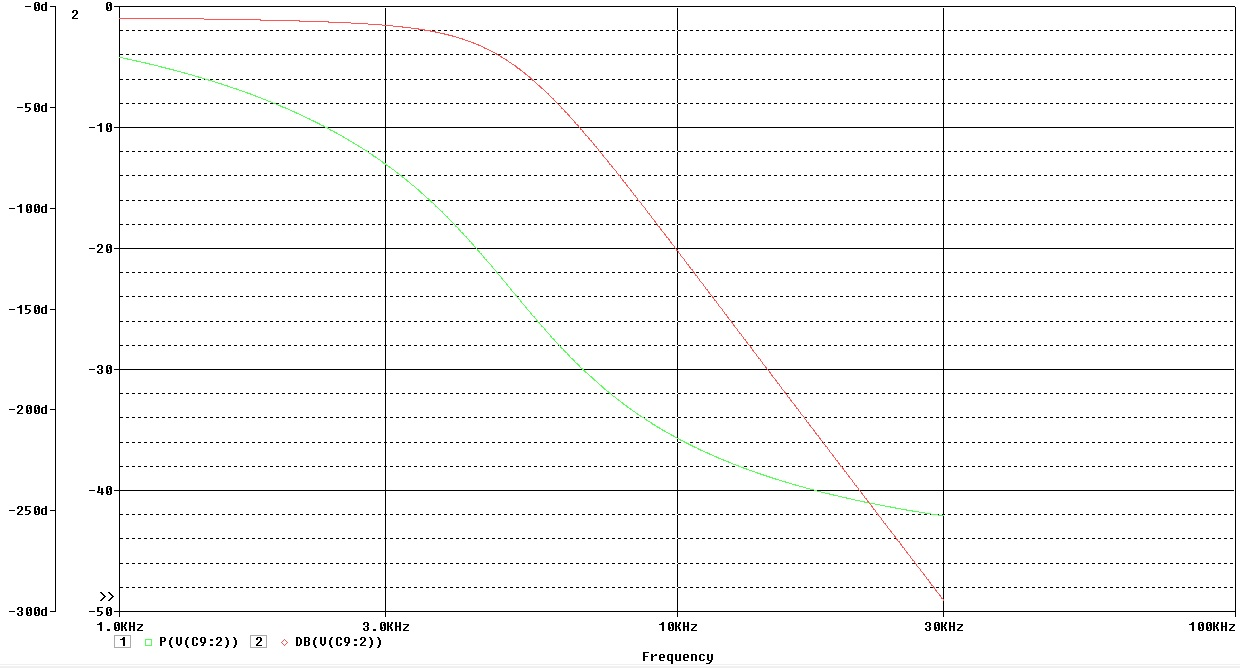
\includegraphics[scale=0.5]{Imagens/rfpb.jpg}
 \caption{Frequência e fase para o filtro passa-baixas.}
 \end{figure}
  
A tabela \ref{tFPB} expõe os dados obtidos através da simulação do circuito.

\begin{small}
\begin{table}[H]
\begin{center}
\caption{Dados da simulação para o filtro passa-baixas.}

\begin{tabular}{l|l}
\hline
\hline
$f_c$ & 4726 Hz\\
\hline
Perda de Inserção & 1dB\\
\hline
Atenuação na banda de rejeição & -60dB/déc \\
\hline
Defasagem & $45^o$ \\
\hline
\hline
\end{tabular}

\label{tFPB}
\end{center}
\end{table}
\end{small}

\subsection{FPA}

A resposta em frequência para o filtro passa-altas é mostrada na figura \ref{fRFPA}.

\begin{figure}[H]
 \centering
 \label{fRFPA}
 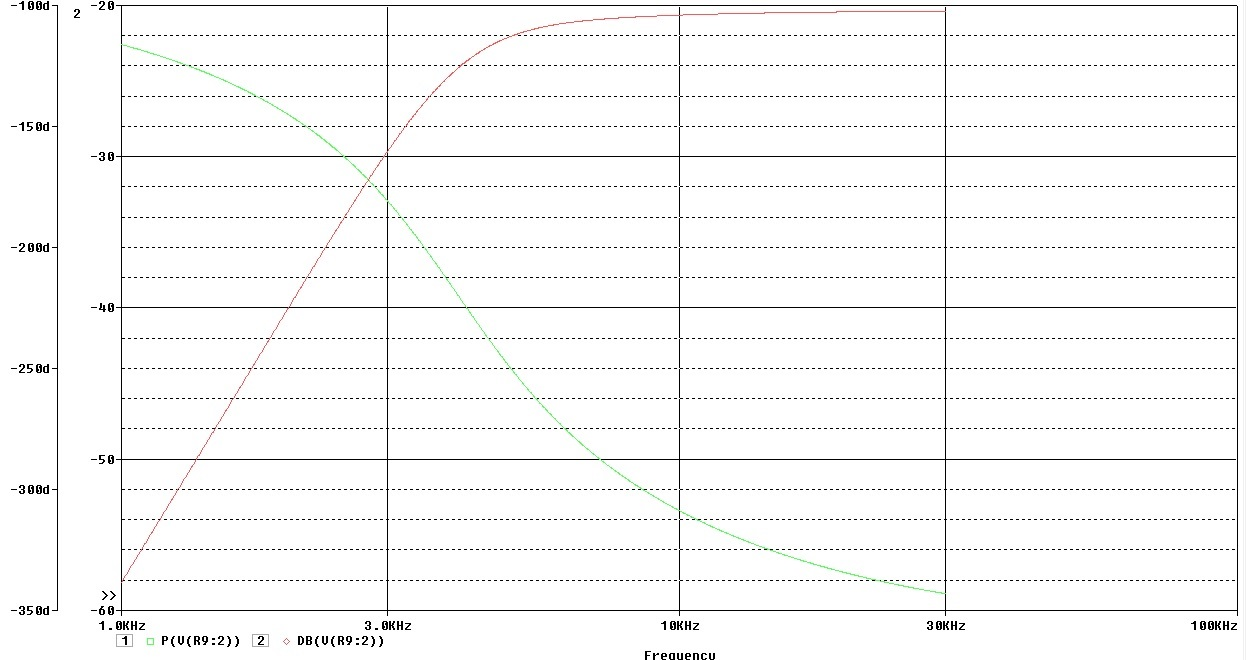
\includegraphics[scale=0.5]{Imagens/rfpa.jpg}
 \caption{Frequência e fase para o filtro passa-baixas.}
 \end{figure}
  
A tabela \ref{tFPA} expõe os dados obtidos através da simulação do circuito.

\begin{small}
\begin{table}[H]
\begin{center}
\caption{Dados da simulação para o filtro passa-altas.}

\begin{tabular}{l|l}
\hline
\hline
$f_c$ & 4217 Hz\\
\hline
Perda de Inserção & 20dB\\
\hline
Atenuação na banda de rejeição & -60dB/déc \\
\hline
Defasagem & $90^o$ \\
\hline
\hline
\end{tabular}

\label{tFPA}
\end{center}
\end{table}
\end{small}

\subsection{FPF Cascata}

A resposta em frequência para o filtro passa-faixa é mostrada na figura \ref{fRFPF1}.

\begin{figure}[H]
 \centering
 \label{fRFPF1}
 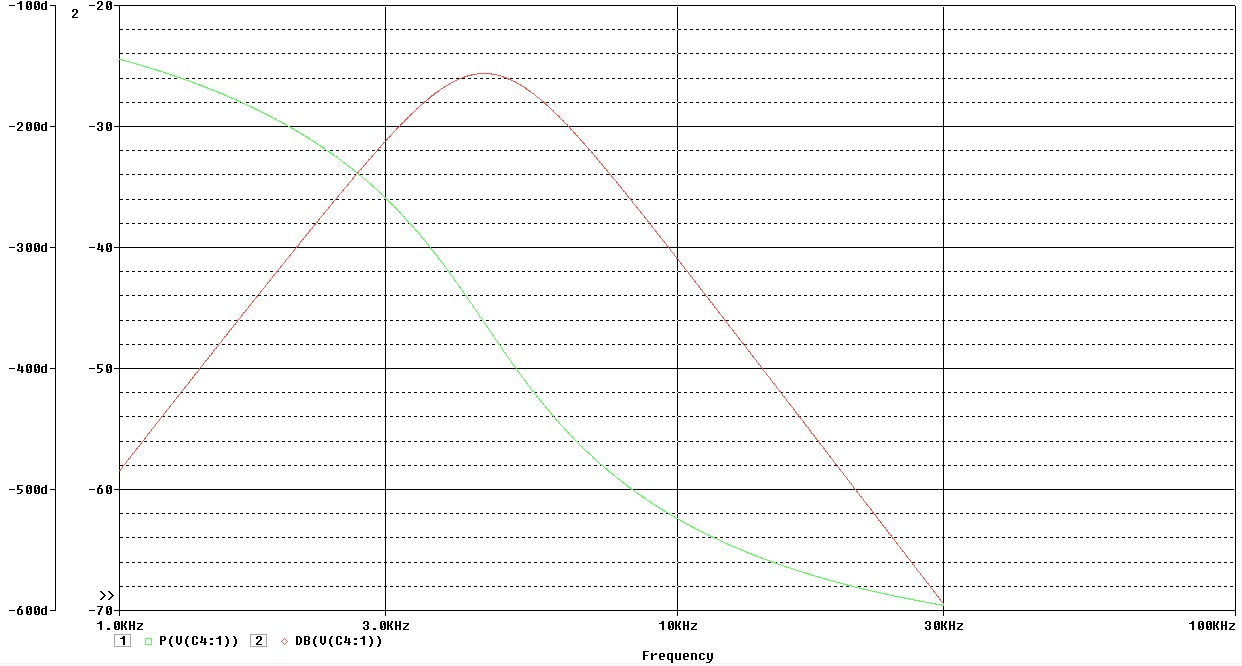
\includegraphics[scale=0.5]{Imagens/rfpf1.jpg}
 \caption{Frequência e fase para o filtro passa-faixa em cascata.}
 \end{figure}
  
A tabela \ref{tFPF1} expõe os dados obtidos através da simulação do circuito.

\begin{small}
\begin{table}[H]
\begin{center}
\caption{Dados da simulação para o filtro passa-faixa em cascata.}

\begin{tabular}{l|l}
\hline
\hline
$f_c$ & 4680 Hz\\
\hline
BW & $2510 Hz$\\
\hline
Perda de Inserção & 25 dB\\
\hline
Atenuação na banda de rejeição & -60dB/déc \\
\hline
Defasagem & $-20^o$ a $-70^o$\\
\hline
\hline
\end{tabular}

\label{tFPF1}
\end{center}
\end{table}
\end{small}

\subsection{FPF}

A resposta em frequência para o filtro passa-faixa é mostrada na figura \ref{fRFPF2}.

\begin{figure}[H]
 \centering
 \label{fRFPF2}
 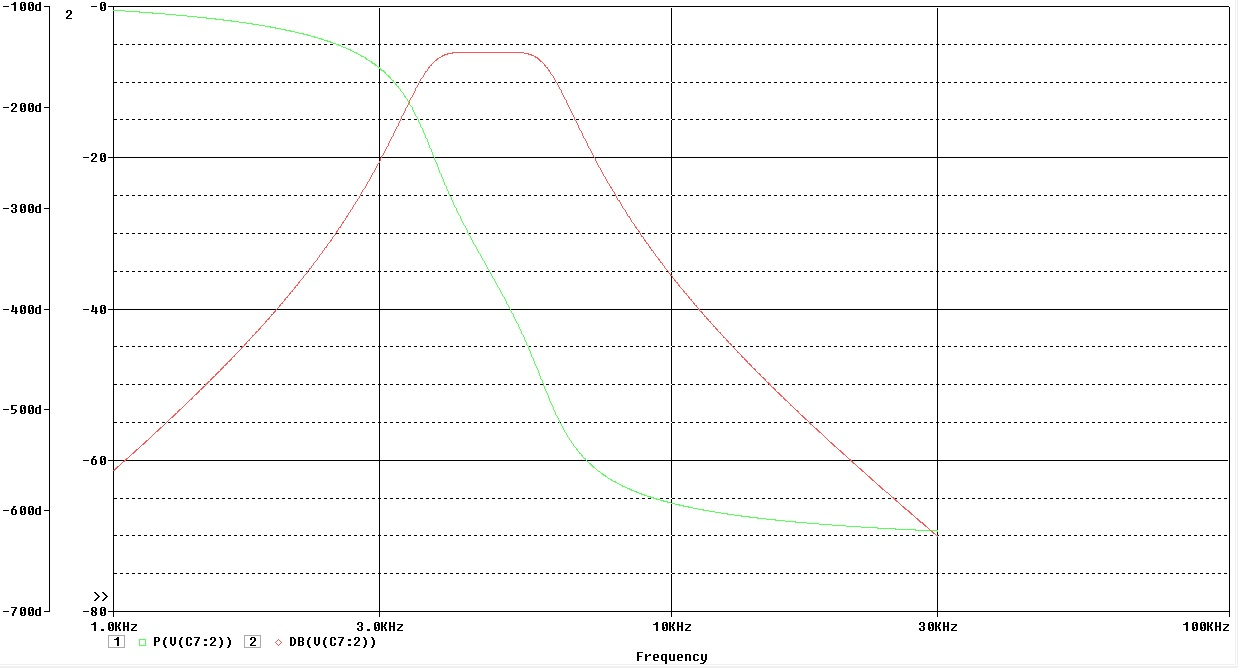
\includegraphics[scale=0.5]{Imagens/rfpf2.jpg}
 \caption{Frequência e fase para o filtro passa-faixa.}
 \end{figure}
  
A tabela \ref{tFPF2} expõe os dados obtidos através da simulação do circuito.

\begin{small}
\begin{table}[H]
\begin{center}
\caption{Dados da simulação para o filtro passa-faixa.}

\begin{tabular}{l|l}
\hline
\hline
$f_c$ & 4850 Hz\\
\hline
BW & $2510 Hz$\\
\hline
Perda de Inserção & 4 dB\\
\hline
Atenuação na banda de rejeição & -60dB/déc \\
\hline
Defasagem & $-20^o$ a $-70^o$\\
\hline
\hline
\end{tabular}

\label{tFPF2}
\end{center}
\end{table}
\end{small}